\section{Évolution d'un modèle de programmation : OpenMP}\label{sec:context:openmp}

OpenMP~\cite{openmp45} est le standard de-facto pour exploiter les machines parallèles à mémoire partagée.

Jusqu'à la version 2.0 incluse, OpenMP ne proposait qu'un nombre restreint de fonctionnalités, principalement tournées vers la parallélisation de boucles régulières.
L'évolution de son utilisation a amené le comité de standardisation d'OpenMP à ajouter le concept de \emph{tâche} à partir de la version 3.0, en s'inspirant de modèles de programmation déjà existants tel que Cilk.
La version 4.0 d'OpenMP étend les tâches pour ajouter les dépendances de données, et introduit le support pour du matériel de plus en plus utilisé : les accélérateurs.
On y voit aussi l'apparition de mécanismes permettant de contrôler le placement des threads, des directives SIMD, ou encore des instructions atomiques.
La version actuelle d'OpenMP est la version 4.5, qui ajoute certaines fonctionnalités aux constructions existantes, et introduit le concept de \emph{taskloop} : des boucles dont les groupes d'itérations forment des tâches indépendantes.
La version en cours de préparation est OpenMP~5.0 ; parmi diverses améliorations, elle devrait notamment ajouter le support d'une interface utilisable par des outils de visualisation de traces d'exécution et de debugging interactif souhaitant se greffer au plus proche d'OpenMP.

Les sections suivantes décrivent les différentes fonctionnalités d'OpenMP, dans l'ordre chronologique où elles sont apparues.

\subsection{Fonctionnement de base}



L'utilisation d'OpenMP repose sur deux ensembles de fonctionnalités : le premier est accessible à travers l'utilisation de |pragma| (des directives de compilation) dans le code, et le second est accessible à travers une API dédiée.
OpenMP a été pensé dès le départ comme un modèle \emph{fork-join} (illustré sur la figure~\ref{fig:context:fork-join})

\begin{figure}[ht]
  \centering
  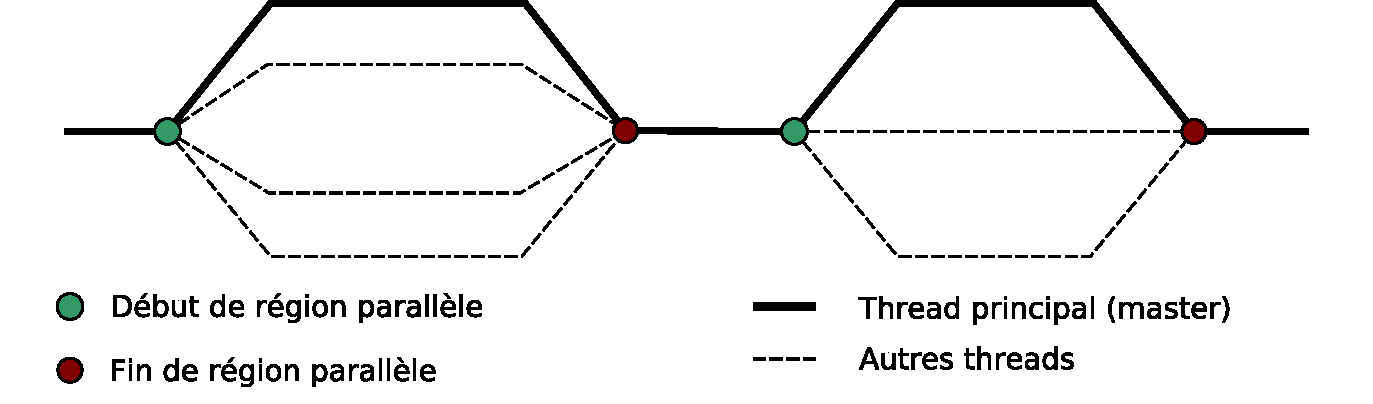
\includegraphics[width=\textwidth]{fork-join}
  \caption{Ligne de vie d'un programme dans un modèle fork-join}\label{fig:context:fork-join}
\end{figure}

Le modèle fonctionne de la manière suivante : le programme est exécuté séquentiellement jusqu'à la rencontre d'une région parallèle (|pragma omp parallel|, comme illustré dans le listing~\ref{lst:context:openmp:parallel}).
À partir de là, plusieurs threads sont créés (ou réutilisés) pour exécuter le bloc de code suivant en parallèle.
Cet ensemble de threads forme une \emph{team} de threads pour la région parallèle.
À la fin de la région parallèle, tous les threads se synchronisent et l'exécution séquentielle est reprise.
Le programmeur peut contrôler combien de threads sont utilisés dans la \emph{team} créée lors de l'entrée dans la région parallèle.

Pour complémenter les fonctionnalités au niveau du langage, OpenMP propose également plusieurs fonctionnalités à travers une API.
Il est possible par exemple de récupérer dynamiquement le nombre total de threads, l'indice du thread courant, ou encore d'ajuster l'ordonnanceur de boucles.

%\noindent
%\begin{minipage}{0.40\textwidth}
\begin{lstlisting}[language=c++,caption=Région parallèle minimale,label=lst:context:openmp:parallel]
int main()
{
  #pragma omp parallel
  {
    // Code à exécuter en parallèle
  }
  return 0;
}
\end{lstlisting}
%\end{minipage}
%\hfill
%\begin{minipage}{0.55\textwidth}
%\end{minipage}


Lors de l'exécution de l'application c'est un programme spécifique - le \emph{support exécutif} qui est en charge de l'équilibrage de charge, et de l'affectation du "travail" aux différents threads.
Si le langage OpenMP est standard et bien défini, les performances dépendent directement du support exécutif.



\subsection{Boucles}

L'une des constructions de partage de travail - ou \emph{worksharing construct} - est la boucle.
Exprimée au moyen d'un |pragma omp for|, elle permet d'indiquer que la boucle à laquelle est attaché le pragma doit être exécutée en parallèle.

Les itérations de la boucle peuvent être réparties sur les différents cœurs de calcul de différentes manières :
\begin{description}
  \item [statiquement :] chaque cœur se voit attribuer un nombre prédéfini d'itérations, typiquement $N/P$ avec $N$ le nombre d'itérations et $P$ le nombre de processeurs. Dans ce genre de cas le compilateur peut directement prendre en charge le découpage.
  \item [dynamiquement :] l'attribution d'une itération, ou d'un groupe d'itérations (\emph{chunk}) se fait lors de l'exécution du programme par le support exécutif. Cela permet notamment de pouvoir faire de l'équilibrage de charge si toutes les itérations ne sont pas parfaitement régulières.
\end{description}
Il existe d'autres options pour contrôler la taille des groupes d'itérations, voire faire varier la taille de ces groupes au fur et à mesure de l'exécution.
Le programmeur a bien sur un contrôle total sur ces options, soit directement dans le code à l'aide de clauses (|schedule|), soit lors de l'exécution via des fonctions de l'API.

Le listing~\ref{lst:context:openmp:parallel-for} illustre la parallélisation d'une boucle simple effectuant l'initialisation d'un tableau. Avec 40 itérations, 4 threads demandés, et un |schedule| statique, chaque thread se verra donc attribuer 10 itérations.

\begin{lstlisting}[language=c++,caption=Exemple d'utilisation d'un for,label=lst:context:openmp:parallel-for]
#define SIZE 40
int main()
{
  double tableau[SIZE];
  #pragma omp parallel num_threads(4)
  {
    #pragma omp for schedule(static)
    for (int i = 0; i < SIZE; i++) {
      tableau[i] = i;
    }
  }
  return 0;
}
\end{lstlisting}

Cette construction existe depuis les toutes premières versions d'OpenMP.


\subsection{Tâches}

Les modèles de programmation à base de tâches permettent d'exprimer du parallélisme à grain fin. L'un des avantages majeurs de ce modèle est qu'il permet au support exécutif d'assigner dynamiquement les différentes tâches, s'adaptant ainsi très bien aux déséquilibrages de charge. Il permet également de composer très facilement des parties de code avec des caractéristiques différentes.

Une \emph{tâche} OpenMP peut être vue comme la plus petite \emph{quantité de travail} qu'un thread OpenMP peut exécuter.
Les tâches peuvent être créées par un thread OpenMP et exécutées par n'importe quel thread de la région parallèle.
Comme la création de tâches à l'exécution du programme est beaucoup plus économique que la création et la synchronisation de threads, le développeur peut pousser la parallélisation de son application encore plus loin : il peut considérer la parallélisation de portions de code qui avaient un grain trop fin pour être parallélisées avec des threads.

Dans la version 3.0 d'OpenMP la synchronisation des tâches est effectuée grâce au mot clé |taskwait|, qui indique au support exécutif d'attendre la complétion des tâches générées jusqu'à ce point dans la région parallèle, avant de reprendre l'exécution.
Le développeur de l'application est responsable de la création et de la synchronisation explicite des tâches, mais c'est le support exécutif qui est en charge de l'affectation des tâches aux threads pendant l'exécution du programme.

Le listing~\ref{lst:context:openmp:taskwait} illustre ce concept avec un exemple très simple initialisant un tableau en parallèle.

\begin{lstlisting}[language=c++,caption=Création et synchronisation explicite de tâches,label=lst:context:openmp:taskwait]
#include <stdio.h>
int main()
{
  double tableau[2];
  #pragma omp parallel num_threads(2)
  {
    #pragma omp task shared(tableau)
    {
      tableau[0] = 0;
    }
    #pragma omp task shared(tableau)
    {
      tableau[1] = 1;
    }
    #pragma omp taskwait
    #pragma omp task shared(tableau)
    {
      printf("Tableau : {%f, %f}\n", tableau[0], tableau[1]);
    }
  }
  return 0;
}
\end{lstlisting}


La version 4.0 d'OpenMP~\cite{openmp40} pousse le concept de tâche plus loin en ajoutant le mot clé |depend|, spécifiant les modes d'accès de chaque variable partagée utilisée par la tâche pendant son exécution.
Le mode d'accès peut être |in|, |out|, ou |inout| selon que la variable correspondante soit respectivement lue comme entrée, écrite en sortie, ou à la fois lue et écrite par la tâche en question.
Cette information peut ensuite être traitée par le support exécutif pour décider si une tâche est prête à être exécutée ou s'il faut d'abord attendre la complétion d'une ou plusieurs autres tâches, ce qui permet de s'affranchir d'une synchronisation par |taskwait| dans énormément de cas.

Le listing~\ref{lst:context:openmp:taskdep} donne un exemple de tâches avec dépendances, où la variable |foo| est initialisée puis affichée.

\begin{lstlisting}[language=c++,caption=Exemple de tâches avec dépendances,label=lst:context:openmp:taskdep]
#include <stdio.h>
int main()
{
  int foo;
  #pragma omp parallel num_threads(2)
  {
    #pragma omp task shared(foo) depend(out: foo)
    {
      variable = 2;
    }
    #pragma omp task shared(foo) depend(inout: foo)
    {
      printf("Foo : %i\n", foo);
    }
  }
  return 0;
}
\end{lstlisting}

La dernière extension aux tâches a vu le jour dans OpenMP~4.5, qui introduit la notion de \emph{priorité} sur les tâches, permettant d'aider le support exécutif à choisir quelle tâche prête exécuter en priorité.

\subsection{Vectorisation}

Nous avons vu dans la section~\ref{sec:context:numa:simd} que les processeurs disposent d'instructions vectorielles - \emph{SIMD} - depuis le début des années 2000.
Avec la multiplication des architectures et de la taille des registres, beaucoup de nouvelles instructions spécifiques à certaines tailles de registre sont apparues.

Si la vectorisation automatique n'est pas possible, il est coûteux pour le programmeur de modifier son code en fonction des architectures.
OpenMP~4.0 tente de résoudre ce problème par l'introduction d'une construction |simd|, qui permet au programmeur d'indiquer quelles parties de son code peuvent être vectorisées et avec quelles contraintes (longueur maximale, alignement, quelles sont les variables d'itérations, ...).
On peut voir ça comme une façon portable d'indiquer au compilateur comment vectoriser un code applicatif complexe.

Le listing~\ref{lst:context:openmp:simd}, donné comme exemple par~\cite{HPCToday} illustre la parallélisation et la vectorisation d'une opération complexe sur un tableau.
Dans cet exemple les itérations seront réparties sur les différents threads, et au sein de chaque thread le code sera vectorisé.
Du aux dépendances entre les différentes itérations de la boucle, le compilateur ne pourrait pas vectoriser automatiquement ce code.
En revanche le programmeur peut identifier que pour une itération donnée, deux lectures sont faites à 18 cases d'écart dans le tableau. Une vectorisation utilisant un vecteur de taille inférieure ou égale à 18 est donc possible sans changer la sémantique du programme.
L'utilisation de la clause |safelen| permet d'indiquer cela au compilateur.


\begin{lstlisting}[language=c++,caption=Vectorisation d'une opération complexe sur des tableaux,label=lst:context:openmp:simd]
#define N 1000000
float x[N][N], y[N][N];
#pragma omp parallel
{
  #pragma omp for
  for (int i = 0; i < N; i++) {
    #pragma omp simd safelen(18)
    for (int j = 18; j < N-18; j++) {
      x[i][j] = x[i][j-18] + sinf(y[i][j]);
      y[i][j] = y[i][j+18] + cosf(x[i][j]);
    }
  }
}
\end{lstlisting}



\subsection{Accélérateurs}

La majorité des supercalculateurs intègre des accélérateurs (comme des GPUs).
L'exploitation de ces accélérateurs impose parfois l'usage d'un langage spécifique au constructeur (tel que Cuda).

Bien que des standards, comme OpenCL~\cite{Stone2010}, existent pour cibler différents types d'accélérateurs, cibler ce type d'architecture via OpenMP était impossible.

OpenMP~4.0 introduit la construction |target|, qui permet de demander au compilateur de créer une tâche à partir de la région de code sélectionnée, qui peut ensuite être exportée sur accélérateur.
Plusieurs clauses permettent de spécifier des dépendances, ainsi que l'ensemble des données à transférer vers l'accélérateur, et l'ensemble des données à rapatrier depuis l'accélérateur à l'issue des calculs.

\begin{lstlisting}[language=c++,caption=Addition sur un accélérateur,label=lst:context:openmp:target]
#define SIZE 40
int main()
{
  double tableau[SIZE];
  #pragma omp target map(tofrom: tableau[0:SIZE])
  {
    for (unsigned i = 0; i < SIZE; i++)
      tableau[i] = i;
  }
  return 0;
}
\end{lstlisting}


Si la norme indique le support de plusieurs accélérateurs, ils doivent cependant être tous du même type, et la transformation du code C/C++/Fortran du bloc est laissée au compilateur implémentant la norme.
Dans le cas d'utilisation d'appels de fonctions, le programmeur doit indiquer qu'elles disposeront d'une définition pour l'\emph{hôte} et l'\emph{accélérateur} via une construction |declare target|.

Ces contraintes font qu'aujourd'hui la construction n'est pas clairement adoptée telle quelle par les programmeurs d'architectures hétérogènes.

\subsection{Placement des threads}

La version~4.0 d'OpenMP voit aussi l'ajout d'un ensemble de fonctionnalités ayant pour but de donner du contrôle au programmeur sur le placement des threads OpenMP sur la topologie physique de la machine.

Le premier ajout est celui du concept de \emph{places} : il s'agit d'un moyen de représenter des emplacements physiques sur lesquels les threads OpenMP peuvent venir se placer, et permet d'indiquer au support exécutif quelles ressources physiques lui sont disponibles.
Le contrôle de la sélection des \emph{places} se fait via la variable d'environnement |OMP_PLACES|.
Elle peut être une liste précise d'indices de cœurs physiques, ou prendre la valeur d'éléments plus génériques de la machine tels que \emph{sockets} ou \emph{cores}.

Il n'y a pas de dépendance entre le nombre de threads dans une région parallèle (spécifié par |OMP_NUM_THREADS|) et la liste des \emph{places} : il peut y avoir plus de threads que de \emph{places} ou inversement, sans que cela empêche l'exécution du programme.

Le second ajout est la possibilité de spécifier la manière dont sont affectés les threads aux \emph{places}, à l'aide de la variable d'environnement |OMP_PROC_BIND|.

À travers cette option il est possible de demander à ce que les threads soient groupés proches les uns des autres sur les \emph{places} (\emph{close}), ou au contraire les plus éloignés possible (\emph{spread}).
S'il est possible d'expérimenter avec ces valeurs, il faut absolument éviter de désactiver le placement fixe des threads (valeur \emph{false}) : cela permettrait au système d'exploitation de migrer les threads d'une région parallèle sur les différentes places, ce qui pourrait entraîner une perte de la localité des données, et donc une dégradation des performances.
Une bonne valeur par défaut dans un contexte NUMA est de positionner |OMP_PROC_BIND| à \emph{true}, afin de fixer les threads sur les cœurs.
Il suffit ensuite d'utiliser l'expressivité des \emph{places} pour spécifier exactement quels cœurs utiliser.

